\section{\name{} Design}\label{sec:design}

\name{} is an orchestration system that achieves the flexibility of ad-hoc
orchestration without compromising the scalability, fault-tolerance, and
execution guarantees of centralized orchestrators. It does so by placing
decentralized orchestration logic in a library that runs in-situ with FaaS
fucntions and leverages a scalable consistent storage service for coordination
and deduplication. Similar to many centralized orchestrators, \name{} workflows
are modeled as a directed execution graph where nodes represent user-defined
FaaS functions and each edge represents an invocation of one function (incoming
edge) with the output of one or more other functions (outgoing edges).

An \name{} graph may include fan-outs, where output from a node is used to
invoke several functions or split up and ``mapped'' multiple times on the same
function. Each such branch may be taken conditionally, based on the output value
or dynamic states of the graph. Execution graphs may also contain fan-ins, where
the outputs of multiple nodes are used to invoke a single aggregate function.
Cycles are also supported and each iteration through a cycle is a different
invocation of the target function.

\subsection{Architecture}\label{sec:design:architecture}

\begin{figure*}[t!]
	\centering
	\begin{subfigure}[t]{0.8\textwidth}
	\centering
		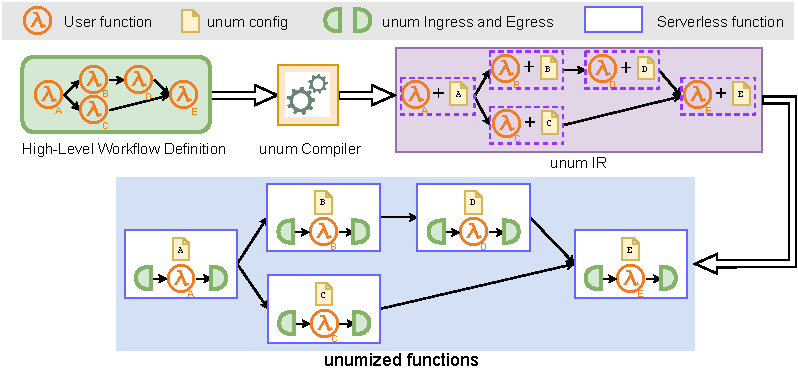
\includegraphics[width=0.8\columnwidth]{figures/unum-arch-compile-time.pdf}
		\caption{Serverless workflows form directed graphs. \name{}
		partitions the graph into an intermediate representation where each
		function is embedded with an \name{} configuration that encodes how to
		transition to its immediate downstream nodes. Developers package user
		function, \name{} config and \name{}'s runtime library (a pair of
		ingress and egress components) together to create unumized functions.}
		\label{fig:arch:unum-compile-time}

	\end{subfigure}
	\begin{subfigure}[b]{\columnwidth}
		\centering
		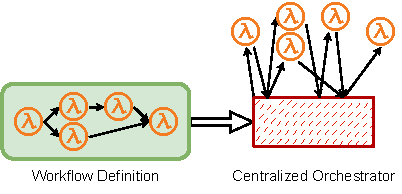
\includegraphics[width=0.8\columnwidth]{figures/unum-arch-centralized.pdf}
		\caption{A typical serverless workflow system drives workflow logic
			using a centralized orchestrator that invokes constituent
			functions and waits for their outputs.}
		\label{fig:arch:centralized}
	\end{subfigure}
	\hfill
	\begin{subfigure}[b]{\columnwidth}
		\centering
		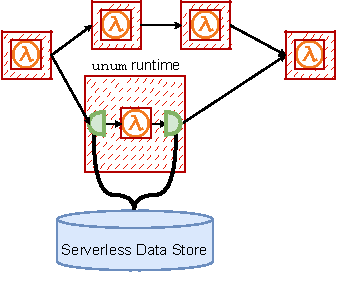
\includegraphics[width=.7\columnwidth]{figures/unum-arch-runtime.pdf}
		\caption{At runtime, \name{} orchestration logic is decentralized and
			runs in-situ with the user functions on an unmodified serverless
			platform. For synchronization and checkpointing,
			\name{} relies exclusively on a standard datastore of choice, such
			as DynamoDB or Cosmos DB.}
		\label{fig:arch:unum-runtime}
	\end{subfigure}
	\caption{\name{}'s Decentralized Orchestration. \name{} partitions
	orchestration logic at compile time and a \name{} runtime runs in-situ
	with user functions to perform only the orchestration logic local to its
	node.}
	\label{fig:arch}
\end{figure*}

Figure~\ref{fig:arch:unum-compile-time} depicts how developers run serverless
workflows using \name{}. Developers write individual functions and describe the
workflow using a high-level workflow language, such as Step Functions'
expression language. An \name{} front-end compiler uses these to extract
portable \name{} IR for each node in the graph and ``attaches'' it to the
function (e.g.\ by placing a file containing the IR alongside the function
code). A platform-specific \name{} linker ``links'' each function with a
platform-specific \name{} runtime library.~\footnote{Since functions are
typically written in dynamic languages, the \name{} library source code is
placed alongside the function and dynamically imported, rather than statically
linking an object file} Developers deploy each linked function along with its IR
to the FaaS platform.  Invoking the first function in the graph (e.g.\ using an
HTTP or storage trigger) starts a workflow.

The runtime library is composed of an ingress and egress component that run
before and after the user-defined function and unwrap and wrap the results of
the function in \name{} execution state, respectively
(Figure~\ref{fig:design:unum-request}). The ingress component coalesces input
data from each incoming edge (e.g.\ in a fan-in), resolves input data if passed
by name rather than by value, and passes the input value to the function. The
egress component uses the function's result to invoke the next function(s),
enforces execution semantics using checkpoints, performs coordination with
sibling branches in fan-in, and deletes intermediate states no longer needed for
the workflow, executing the workflow in-situ with the functions, in lieu of a
centralized orchestrator (Figure~\ref{fig:arch:unum-runtime}).

\subsection{\name{} Intermediate Representation}\label{sec:design:ir}

\begin{table}[t]
  \centering
  \begin{tabular}{|m{0.45\linewidth}|m{0.45\linewidth}|}
    \hline
  \texttt{Invoke(Fn)} & Queue a single invocation of a function.\\
    \hline
  \texttt{Map(Fn)} & Queue one function invocation for each element in the current function's result.\\
    \hline
  \texttt{FanIn(Set, Size, Fn)} & Queue a fan-in to a function using the provided coordination set object and size.\\
    \hline
  \texttt{Pop} & Pops the top frame of the execution state stack (passed via \name{} requests). \\
    \hline
  \texttt{Next} & Increments the current execution state frame's iteration counter.\\
    \hline
  \texttt{CreateSet(Name)} & Creates a coordination set object in the datastore with the provided name.\\
    \hline
  \end{tabular}
  \caption{\name{} intermediate representation instructions.}
  \label{table:design:irschema}
\end{table}

\begin{figure}[t]
    \centering
    \begin{minted}[
        frame=single,
        fontsize=\scriptsize
        ]{rust}
struct InvocationRequest {
  data: Vec<DatastoreObjectName>,
  workflowId: String,
  fanOut: Stack<FanOut>,
}

struct RequestData {
  reference: DatastoreObjectName,
  value: Option<Value>
}

struct FanOut {
  index: usize,
  size: usize,
  iteration: usize,
}
    \end{minted}
    \caption{An \name{} request wraps the outputs of parent nodes with execution
state that allows function invocations to be named uniquely and assists in
coordinating fan-ins. \name{} IR instructions can reference this metadata and
modify it for subsequent functions.}
    \label{fig:design:unum-request}
\end{figure}

The \name{} intermediate representation (IR) is designed to allow encoding of
common workflow patterns but is low-level enough to also support less uncommon
patterns.

Each function's IR includes the function's name and a sequence of instructions
(Table~\ref{table:design:irschema}). Instructions direct the runtime to invoke
functions and operate on state metadata passed between functions in
\name{}-wrapped function inputs (Figure~\ref{fig:design:unum-request}).

The egress component, which receives the function's user-code output, executes
the IR and uses it to determine which next steps to take. An invocation can be
protected by a conditional---a boolean expression that operates on the
invocation request and the current function's output. \name{}'s IR provides
three kinds of invocations:

\begin{itemize}
  \item \textbf{Invoke} simply invokes the named function using the
        current functions output.
  \item \textbf{Map} treats the current function's output as iterable data
        (e.g.\ a list) and invokes the named function once for each item in the
        output.
  \item \textbf{FanIn} invokes the named function using the current function's
        output along with the outputs of all other functions fanning into the
        same node. Fan-in requires coordination among multiple functions and is
        described in detail in \S\ref{sec:design:fanin}.
\end{itemize}

When multiple invocations occur, either using multiple instructions or a single
\texttt{Map} invocation, each of the invocations adds a fan-out frame to the
invocation request's fan-out stack. This allows different invocations of the
same function to be differentiated for naming (\S\ref{sec:design:naming}) and to
coordinate fan-in (\S\ref{sec:design:fanin}).

The IR also includes instructions for manipulating the \name{} request data and
an instruction that creates a new coordination set, typically for use in later
nodes to coordinate fan-in (\S\ref{sec:design:fanin}) or garbage collection
(\S\ref{sec:design:garbage}).

This IR is sufficient to represent basic patterns, as well as more complex
fan-in patterns (described in \S\ref{sec:design:fanin}).

\paragraph{Chain \& Fan-out.}
\name{} encodes passing the output of a function to one (chaining) or more
(fan-out) subsequent functions, simply, with one or more calls to the
\texttt{Invoke} instructions.

\paragraph{Map.}
Applications may also perform the same operation on each component of a
function's output. For example, an application may unpack an archive of
high-resolution images in one function and perform compression on each of the
resulting images. \name{}'s \texttt{Map} invocation pass each element from the
function's output to a different invocation of the same function.

\paragraph{Branching.}
Applications may need to invoke different functions based on runtime conditions
(e.g., the output of a function). For instance, an application may first
validate that a user-uploaded photo is a valid JPEG. If it is, it invokes, e.g.,
one of the patterns above, otherwise it notifies the user of the error.
\name{}'s invocation instructions are optionally protected by a conditional
expression that has access to the function output and execution metadata
(Figure~\ref{fig:design:unum-request}).

\subsection{Execution Guarantees Using Checkpoints}\label{sec:design:execution}

FaaS platforms guarantee at-least once execution of individual functions
invocations. As a result, an invocation may result in more than one execution of
the function and, because functions may be non-deterministic, this can result in
multiple different results for the same invocation.

One of the benefits of an orchestrator is to provide strong workflow execution
semantics. While individual functions within a workflow may execute more than
once, an orchestrator chooses a single result of these executions to use as
input for all downstream functions. At the end of the workflow, the result is
consistent with an execution of the workflow where each function invocation
executed \emph{exactly-once}.

Because centralized orchestrators interpose on all communication between
workflow stages and are solely responsible for moving a workflow state machine
forward, providing these execution guarantees is conceptually straightforward
(though doing scalably and tolerant of orchestrator faults may not be
straightforward).

A key challenge for \name{} is to provide the same semantics without
centralizing orchestration. Moreover, because failures and, thus, retries are
the exception, not the rule, \name{} should provide these semantics without
expensive coordination---function instances should be able to proceed without
blocking to avoid unnecessary resource usage and cost in the common case.

\name{} leverages two key insights to achieve these semantics.  First, it is ok
for different executions of the same function invocation to return different
results as long as \name{} ensures downstream functions are always invoked with
exactly one of those results. Second, a workflow's output is \emph{correct} even
if a function invocation is requested more than once, as long as the invocations
uses the same input, since additional, but identical, invocations are
indistinguishable from additional executions.

The \name{} library employs an atomic \texttt{create\_if\_not\_exists} operation
in the serverless datastore to \emph{checkpoint} exactly one execution of each
function invocation. The egress component of the \name{} library attempts to
write the result of the function to a checkpoint object in the datastore. If
such a checkpoint already exists, a concurrent or previous execution of the
invocation must have already completed and the operation will fail. To invoke
downstream functions, the egress component \emph{always} uses the value stored
in the checkpoint, rather than the result of the recently completed function.
Essentially, \name{} ``commits'' to result of the first successful execution of
the function.

As a further optimization, the ingress component in the \name{} library checks
for the checkpoint object before executing the user-defined function. If the
object exists, it bypasses the user-defined function and passes the checkpoint
value directly to the egress component to invoke downstream functions. This is
not necessary for correctness (and it is, of course, possible for the checkpoint
to be added after a concurrent execution checks for its existence in the ingress
component) but helps reduce computation that we know will go unused.

\begin{figure}
\begin{minted}[
    frame=single,
    fontsize=\scriptsize
    ]{python}
def ingress(self, function):
    ...
    result = datastore_get(self.checkpoint_name):
    if result:
        self._egress(result)
    else:
        self.egress(function.handle())

def egress(self, result):
    ...
    if not datastore_atomic_add(self.checkpoint_name, result):
      result = datastore_get(self.checkpoint_name)
    self._egress(result)
    ...

def _egress(self, result)
    for f in next_functions:
        faas.async_invoke(f, result)
\end{minted}
\caption{Pseudo-code showing \name{}'s checkpointing mechanism. As different
executions of a function may return different results, \name{}'s egress
component checkpoints the first successful execution using an atomic add
datastore operation. All subsequent executions will uses this committed value
rather than the result their own execution returned.}
\label{fig:design:checkpoint}
\end{figure}

\subsubsection{Fault Tolerance}

\name{}'s checkpointing mechanism ensures that while faults may occur at any
point during the execution of a function's user code or the \name{} library, and
while downstream functions may be invoked multiple times by different executions
of the same invocation, a single value is always used to invoke downstream
functions.

If there is a fault after the user code completes but before creating the
checkpoint, its value is ignored (indeed, never seen) by other attempts to
execute the function and another execution's value will be used to invoke
downstream functions.  If the ``winning'' function crashes after creating a
checkpoint, and before invoking some or all downstream functions, other
executions will use the checkpoint value to invoke downstream functions.
Finally, even if multiple executions invoke some or all downstream functions,
execution guarantees are still satisfied as these invocations will have
identical inputs.

\subsection{Fan-in Patterns}\label{sec:design:fanin}

In fan-in patterns, the results of multiple nodes are used to invoke a single
target node. Such patterns are a particular challenge for decentralized
orchestration because invoking the target function cannot happen until all
branches complete, but there is no centralized orchestrator to wait for this
condition. Designating one of the dependent functions as a coordinator for the
fan-in would address this directly, however there is no guarantee that branches
for a fan-in complete soon after each other, incurring a potentially large
resource cost to do virtually no work, or exceeding platform enforced time
limits on function invocations. Moreover, functions typically cannot communicate
with each other directly, so it is not obvious how other branches would notify
this coordinator of their completion.

\name{}, instead, leverages the same insight as checkpoints---the datastore
provides strong consistency that can serve as a coordination point. Rather than
designate a single branch function as the coordinator, all branches are
empowered to invoke the fan-in function once all other branches have completed.
To determine this condition, branches in a fan-in add the name of their
checkpoint object to a shared ``Set'' in the datastore. Any branch that reads a
the set with size equal to the total number of branches invokes the target
function using all the branches' checkpoints as input.

Importantly, functions do not wait for any other to complete. As long as all
functions complete eventually (in other words, they run at-least once),
\emph{some} function will read a full set and invoke the fan-in target function.
More than one function may observe this condition, resulting in multiple
invocations, but these invocations will be identical and are handled as spurious
executions of the same invocation (\S\ref{sec:design:execution}).

In order to perform this coordination, branches must know the branching
factor---the size of the set. The \texttt{FanIn} instruction includes this size,
which is either specified explicitly, or using a variable from the invocation
request, commonly the fan-out size.


This enables more patterns that commonly arise in applications:

\paragraph{Aggregation}
After processing data with many parallel branches, applications commonly want to
aggregate results. For example, to build an index of a large corpus, the
application might process chunks in parallel and the aggregate the results.
Aggregation is a common pattern to join back multiple parallel functions, by
invoking a single ``sink'' function with the outputs from a vector of functions.

\paragraph{Fold}
\texttt{fold} sequentially applies the same function on the outputs of a vector
of source functions, while aggregating with the intermediate results of running
the function so far. For example, a video encoding application might encode
chunks in parallel and then concatenate the results in order: concatenating
chunk 1 and 2, then concatenating chunk 3 to chunk [1--2], and so on.
\texttt{fold} is an advanced pattern that is not supported by all existing
systems (e.g., AWS Step Functions do not support \texttt{fold}) but is
expressible in \name{}.


\subsection{Garbage Collection}\label{sec:design:garbage}

Both checkpointing, to provide correct workflow execution semantics, and fan-in
require storing intermediate data in the datastore. This poses a garbage
collection challenge.

Both checkpoints and fan-in coordination sets may be numerous in a workflow and only
temporally useful. Deleting checkpoints or bitmaps too early can compromise
execution guarantees and deleting too late incurs unnecessary storage charges
from the datastore. \name{} deletes checkpoints and bitmaps as soon as they are
no longer needed for execution correctness.

\subsubsection{Checkpoint Collection}

A checkpointing node does not know when \emph{its} checkpoint is no longer
necessary.  If it deletes its checkpoint after invoking subsequent functions but
before completing, it may crash and the FaaS platform may re-execute it,
yielding a potentially inconsistent result. However, downstream nodes know that
once they have committed to a value by checkpointing, previous checkpoints are
no longer necessary to ensure their own correctness. Once a node has committed
to some particular output, future invocations, even with \emph{different} inputs
will produce the same output, as the node will \emph{always} use the checkpoint
value.

In particular, \name{} collects checkpoints by relaxing the constraint that
nodes always output the same value. Instead, they must only output the same
value until all subsequent nodes have committed to their own outputs.

This means that, in non-fan-out cases, once a node checkpoints its result, it
can delete the previous checkpoint.

Note that \name{} runtime implementations delay garbage collection until after
invoking next functions, sacrificing some storage overhead in favor of
minimizing end-to-end latency for a workflow.

Fan-out cases are more complicated because deleting the checkpoint must wait
until all branches have committed to an output. \name{} repurposes the same
set-based technique from fan-in to collect checkpoints in fan-out cases as well.
The originating node of a fan-out creates a set for branches to coordinate when
to delete its checkpoint. Branches add themselves to the set after checkpointing
their own value. Any node that reads a full set deletes the parent's checkpoint
as well as the set. This guarantees that the parent's checkpoint is deleted and
ensures that all branches have first checkpointed.

Note that it is possible for one of the branches to re-execute \emph{after} the
set has been deleted. This is safe because it is the origin of the fan-out that
creates the set, so a branch's attempt to add itself to a, now, non-existent set
will simply fail.

\begin{minted}[
    frame=single,
    fontsize=\scriptsize
    ]{python}
def egress_fan_out(self, result):
    result = _checkpoint(self, result)
    _do_next(result)

    completion_set_after =
        write_set_read_result(fan_out_gc_set, fan_out_index)
    if all_complete(completion_set_after):
        database_delete(prev_checkpoint)
        database_delete(fan_out_gc_set)
\end{minted}

\subsubsection{Fan-in Set collection}

Deleting sets used for fan-in works much like removing checkpoints---the target
node of a fan-in deletes the set once it has generated a checkpoint. However,
who \emph{creates} the set?

If each branch in the fan-in creates the set if it doesn't already exist, a
spurious execution of one of the branches \emph{after} the fan-in target removes
the original set will create a new one that is never deleted (because it never
fills, and thus the target function is never invoked again). To avoid this,
\name{} places the responsibility to create the set on the node that originates
the \emph{fan-out} at the same level as the target node.

\subsection{Naming}\label{sec:design:naming}

Much of \name{}'s functionality relies on unique naming. A workflow invocation
must be named to differentiate it from other concurrent invocations of the
workflow; functions must be named to invoke them; different invocations of
functions must have different names to uniquely name invocation checkpoints and
coordination sets for fan-in.

Each workflow invocation has a unique name that is passed through the execution
graph. The name is either generated in the ingress to the first function using,
e.g., a UUID library or, when available, is taken from the FaaS platform's
invocation identifier for the first function. This enables functions to have
different names when invoked as part of a specific workflow invocations. The
function's name is either user-defined or determined by the FaaS platform (e.g.\
the ARN on AWS Lambda) and determined at ``compile-time'' (i.e.\ when generating
\name{} IR).

However, this is not sufficient as functions may be invoked multiple times in
the same workflow due to map patterns---which invoke the same function multiple
times over an iterable output---and cycles. Moreover, invocation names must be
determined using local information only. Once running, each function only has
access to it's own code (including the IR) and metadata passed in its input.
Nonetheless a particular invocation must be able to determine its own name for
checkpointing as well as, if it is part of a fan-in, the name of downstream
invocations to coordinate with other branches.

As a result, \name{} names function invocations using a combination of the
global function name, a vector of branch indexes and iteration numbers (taken
from the \name{} request fan-out stack) leading to the invocation, and the
workflow invocation name. Function names are global and the remaining items are
propagated by \name{} in invocation arguments.

During a fan-out pattern (multiple scalar invocations or a map invocation), a
branch index is added to a list in the next functions' input. If the next
function is an ancestor of the current function (a cycle), an iteration field in
the input is incremented. Note that a single iteration field is sufficient even
if there are nested cycles since it is only important that different invocations
of the same function have \emph{different} names, not that the iteration field
is sequential. Thus, a monotonically increasing iteration field is sufficient.

We note that the format of this name is not significant and, importantly, it
need not be interpretable. It must only be deterministic and unique for its
inputs. For example, a reasonable implementation could serialize the inputs and
take a cryptographic hash over the result, guaranteeing uniqueness (with very
very high probably) while preventing names from growing too large to use as
object names.
